\chapter*{Part One: Count Based Language Modeling}
\addcontentsline{toc}{chapter}{Part One}



    % \begin{lstlisting}[style=latexFrameTB, caption={Example of Sleek Template packages usage.}, gobble=8]
    %     \usepackage[english]{babel}
    %     \usepackage[noheader]{packages/sleek}
    %     \usepackage{packages/sleek-title}
    % \end{lstlisting}


\subsection*{Theoretical Problem A}
The assignment is to solve for the maximum likelihood estimate (MLE) of a bigram language model, where the likelihood function is given by

\begin{equation*}
    \prod_{t=1}^{T} p_{\theta_{u,v}}(w_t | w_{t-1})
\end{equation*}

For brevity, I will refer to  $p_{\theta_{u,v}}$ as simply \theta. 

If we define our corpus to consist of many two word pairs, or bigrams, we can re-write the likelihood as

\begin{equation*}
    \prod_{t=1}^{T} \theta^{c(u,v)}
\end{equation*}

where $c(u,v)$ represents the count of how many times the bigram $u,v$ appears in the corpus.

It is convenient to rewrite our function in terms of the log likelihood:
\begin{equation*}
    \sum_{t=1}^{T} c(u,v) * \ln{\theta}
\end{equation*}

We want to maximize the log likelihood in terms subject to the constraint that the probabilities $\theta$ sum to 1:
\begin{equation*}
    \sum_{u,v\in \mathcal{V}} \theta = 1
\end{equation*}

We introduce a Lagrangian multiplier to solve the problem in the form 
\begin{equation*}
    \mathcal{L}(\theta,\lambda) = L(\theta) - \lambda f(\theta)
\end{equation*},
yielding
\begin{equation*}
    \mathcal{L}(\theta,\lambda) = \sum_{t=1}^{T} c(u,v) * \ln(\theta) - \lambda (\sum_{u,v\in \mathcal{V}}\theta -1)
\end{equation*}

Taking the partial derivatives gives the following system of equations:

\begin{equation*}
    \frac{\partial}{\partial \theta} = \frac{c(u,v)}{\theta} - \lambda = 0
\end{equation*}

\begin{equation*}
    \frac{\partial}{\partial \lambda} = \sum \theta - 1 = 0
\end{equation*}

Solve the system of linear equations:

\begin{equation*}
    \theta = \frac{c(u,v)}{\lambda}
\end{equation*}

\begin{equation*}
    \sum \frac{c(u,v)}{\lambda} = 1
\end{equation*}

\begin{equation*}
    \lambda = \frac{1}{\sum c(u,v)}
\end{equation*}

The final solution to the system of equations is the MLE of the bigram model:
\begin{equation*}
    {\hat \theta_{u,v}} = \frac{c(u,v)}{\sum_{u,v\in \mathcal{V}}c(u,v)}
\end{equation*}

\subsection*{Theoretical Problem B}

The assignment is to show that for the case of a unigram language model, given a prior distribution of a Dirichlet distribution, setting all values in parameter vector $\beta$ results in a posterior distribution with mean equal to the Laplace smoothing estimate:

\begin{equation*}
    \hat{\theta}_u = \frac{c(u) + \alpha}{T + \alpha|\mathcal{V}'}
\end{equation*}

The posterior is defined as:
\begin{equation*}
    p(\pi|D;\beta) = \frac{p(D|\pi)p(\pi;\beta)}{p(D)}
\end{equation*}

The density function for the prior is:
\begin{equation*}
    p(\pi;\beta) = \frac{1}{B(\beta)}\prod_{u \in \mathcal{V}}\pi_u^{\beta_u - 1}
\end{equation*}

The likelihood model of $p(D|\pi)$ is given by:
\begin{equation*}
    \prod \pi_u^{c(u)}
\end{equation*}
where we multiply over probabilities over all words in the corpus and account for duplicates with the count term in the exponent. 

Plugging the density function (ignoring the normalizing constant $B(\beta)$) and likelihood model into the posterior gives
\begin{equation*}
    p(\pi|D;\beta) = \frac{\prod \pi_u^{c(u)} * \frac{1}{B(\beta)}\prod_{u \in \mathcal{V}}\pi_u^{\beta_u - 1}}{p(D)}
\end{equation*}

\begin{equation*}
    = \frac{\prod \pi_u^{c(u) + \alpha - 1}}{p(D)}
\end{equation*}

The numerator of this equation is itself a Dirichlet distribution with parameter vector $\beta' = c(u) + \alpha -1$. Because we are changing the observed data by applying a smoothing constant, p(D) becomes trivial. Our result is proportional and the $p(D)$ term does not impact the result. Observe that the expected value of the $\beta'$ distribution is 

\begin{equation*}
    \mathbb{E_{p(\pi|D;\beta')}} = \frac{c(u) + \alpha}{\sum_u^{\mathcal{V}} c(u) + \alpha}
\end{equation*}

We have increased the count of every word in our corpus by $\alpha$, meaning the size of the corpus has increased by $\alpha$ times the number of unique words. This yields

\begin{equation*}
    \mathbb{E_{p(\pi|D;\beta')}} = \frac{c(u) + \alpha}{T + \alpha|\mathcal{V}|} = \theta_u
\end{equation*}
where $T$ is the size of the original corpus. 

\chapter*{Part Two: RNN Language Modeling}
\addcontentsline{toc}{chapter}{Part Two}

\subsection*{Computational Problem A}

In order to determine if a substring is part of BPL, I observe that one must know three quantities: the number of "(", the number of ")", and if an illegal ")" has ever been observed. A ")" is illegal if there is not already a matching "(". 

My hidden state is a column vector with elements \begin{bmatrix}
    "(" count \\ ")" count \\ Illegal \\
\end{bmatrix}. The initial hidden state is given by 
\begin{equation*}
    h_0 = \begin{bmatrix}
        -1 \\ -1 \\ 0 \\
    \end{bmatrix}
\end{equation*}


$x_t$ is a vector representing either "(" or ")", where I map \begin{bmatrix}
    1 && 0 && 0
\end{bmatrix} to  "(" and \begin{bmatrix}
    0 && 1 && 0
\end{bmatrix} to ")".

W and U are unnecessary in my BPL model, and are set to 1. The update function is given by the piecewise function 

\begin{equation*}
    f (x) = 
     \begin{cases} 
        x & x * \begin{bmatrix}
            1 && -1 && 0
        \end{bmatrix}\geq 0 \\
        x + \begin{bmatrix}
            0 \\ 0 \\ 1 \\
        \end{bmatrix} & x * \begin{bmatrix}
            1 && -1 && 0
        \end{bmatrix}< 0 \\
     \end{cases}
  
\end{equation*}

If $h_t \lbrack 0 \rbrack - h_t \lbrack 1 \rbrack $ is 0 and $h_t \lbrack 2 \rbrack $ is 0 then $x_t$ is in BPL.

\subsection*{Vanilla Recursive Neural Network Implementation}

Note to the teaching assistant: I apologize for some weak analysis in the implementation sections. I finished all my code several days ago, but forgot to check the notebook into Github and lost all of my code on Monday night when Chrome crashed. 

My vanilla RNN is essentially a wrapper around either an RNNCell or an LSTMCell. The forward function takes a matrix of input ids representing a batch of sentences, and maps them to an embedding. We then initialize a hidden state to zeros, and iterate over the embeddings symbol by symbol for the 50 symbol sequence. At every step the previous hidden state $h_{t-1}$ is fed back into the model, as well as the next embedding column. 

The perplexity of just my basic model is shown below in Figure \label{firsttry}. 

\begin{figure}[h]
    \centering
    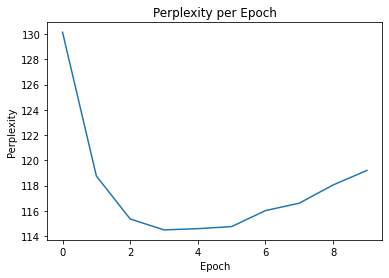
\includegraphics[width=0.4\textwidth]{resources/png/no_bias_1e3.png}
    \noskipcaption{Perplexity of a vanilla RNN over 10 epochs with learning rate 1e-3}
    \label{firsttry}
\end{figure}

The fact that the perplexity gets worse with more training implies that perhaps my optimizer is descending too far, and passing over the maximum for a local maxima. My perplexity rating is far away from the target somewhere in the 70s, so I decided to use a new architecture. Long Short Term Memory or LSTM incorporate a feedback mechanism in addition to the feed-forward method of an RNN. This allows the network to develop connections over longer sequences, potentially allowing for context a vanilla RNN can't achieve. My LSTM has perplexity ~78 as shown in Figure \label{secondtry}.

\begin{figure}[h]
    \centering
    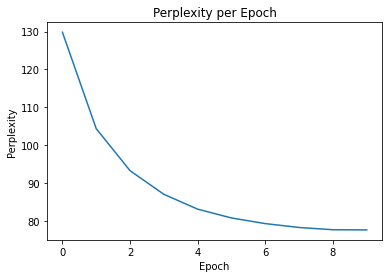
\includegraphics[width=0.4\textwidth]{resources/png/LSTM_05e3.png}
    \noskipcaption{Perplexity of a LSTM RNN over 10 epochs with learning rate 5e-4}
    \label{secondtry}
\end{figure}

\subsection*{Sequence to Sequence Model}
A sequence to sequence model interprets an input sequence through an input neural network called an encoder, and then feeds the final layer of the encoder through a decoder to produce the output sequence. 

My decoder contains a Gated Recurrent Unit, which functions similar to an LSTM but it also can "forget". I chose it because some research indicates GRUs function well on smaller vocabularies ("Empirical Evaluation of Gated Recurrent Neural Networks on Sequence Modeling", Chung et al), although I did not have time to compare to other architectures. 

Additionally I feed the output of my GRU through a linear layer. Empirically this improved my BLEU score by about 0.5, although I do not have great intuition for why. 

The first attempt at a decoder with a single layer GRU and no linear layer achieved a perplexity score in the mid 40s (Figure \label{seq1}).

\begin{figure}[h]
    \centering
    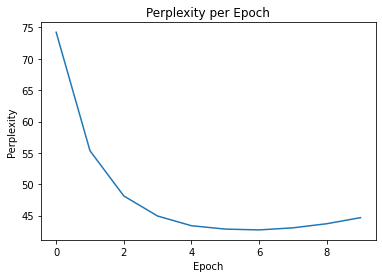
\includegraphics[width=0.4\textwidth]{resources/png/seq2seq1layer.png}
    \noskipcaption{Single layer GRU Decoder perplexity}
    \label{seq1}
\end{figure}

Adding a second GRU layer and the hidden layer resulted in a perplexity in the low 30s, with a BLEU score of 6.83 (Figure \label{seq2}). 

\begin{figure}[h]
    \centering
    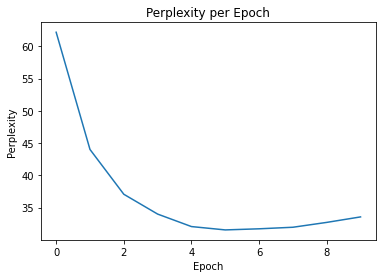
\includegraphics[width=0.4\textwidth]{resources/png/seq.png}
    \noskipcaption{Double layer GRU with linear output Decoder perplexity}
    \label{seq1}
\end{figure}

One thing I noticed about my decoder is the output produces some seemingly unrelated predictions sometimes; the following example is taken from the training data:

    Src :  Tôi đoán các bạn đều đã biết về lịch sử của &quot; đàn quay &quot; trong tiếng Pháp là &quot; <unk> à <unk> &quot;  \hline
    Trg :  I see you &apos;re all up on the history of hurdy-gurdy -- &quot; <unk> <unk> <unk> . &quot; \hline
    Pred:  I think you know what most of the most popular TEDTalks &quot; is &quot; <unk> . &quot; \hline

I looked it up, and there is a sentence about TEDTalks right next to a sentence relating to hurdy-gurdies in the training data. I suspect my batch data is getting entangled. This could be fixed by duplicating some of the training data but with sentences rearranged more randomly, or by playing with the batch size parameters. 

Another error is that the prediction seems to sometimes follow the most likely path, regardless of sentence context. 

Src :  Tôi muốn cho các bạn biết về sự to lớn của những nỗ lực khoa học đã góp phần làm nên các dòng tít bạn thường thấy trên báo . \hline
Trg :  I &apos;d like to talk to you today about the scale of the scientific effort that goes into making the headlines you see in the paper . \hline
Pred:  I want to tell you about the most important thing that you &apos;ve learned in the first place of the brain that works in the front of the job . \hline

In this example it starts out alright, but I suspect addressing a second person after stating "I want to tell you" is more common than "scientific effort...". If my model had beam search, it could explore multiple paths instead of just taking the likely followup to a shorter sequence. 


\chapter*{Appendix}
\subsection*{Vanilla RNN}
\begin{python}
    class RNN(nn.Module):

    def __init__(self, input_size, hidden_size, src_embed, generator, LSTM=True):
      """
      Inputs:
        - `input_size`: a positive integer corresponding to the size of the
            word embeddings
        - `hidden_size`: a positive integer representing the dimensionality of
            the RNN's hidden state vector
        - `src_embed`: an nn.Embedding object representing the lookup table for
            input (source) sentences
        - `generator`: a `Generator` object. Essentially a linear mapping
            followed by a softmax. You should not call it within this class; it
            is called in the SimpleLossCompute class above
      """
      super(RNN, self).__init__()
      # `input_size`, `hidden_size`, and `output_size` are all int.

      self.hidden_size = hidden_size
      self.src_embed = src_embed
      self.generator = generator
      self.use_lstm = LSTM
      # hint: unless you choose to implement the RNN update equations yourself
      #       you will want a `self.rnn` module that does that for you, which
      #       is where the RNNCell/LSTMCell/GRUCell modules come in handy

      self.rnn = nn.RNNCell(input_size, hidden_size, bias=False, device=device)
      self.lstm = nn.LSTMCell(input_size, hidden_size, device=device)


    def forward(self, input_ids):
      """
      Given a sequence of words (represented as IDs), compute and return the
      hidden state at each timestep (equivalently, for each input word).
      Input:
        - `input_ids`: a 2d-tensor of shape
           (batch_size, MAX_SENT_LENGTH_PLUS_SOS_EOS) representing a batch of
           sentences from the dataset (with IDs instead of words)

      Returns:
        - `hiddens`: a 3d-tensor of shape
            (batch_size, MAX_SENT_LENGTH_PLUS_SOS_EOS, hidden_size) representing
            the hidden state of the model at each timestep
      """
      # hint: pay close attention to the shapes of your tensors; you may find
      #       pytorch's `permute()` method for tensors useful

      ### Your code here!
      bsize, fsize = input_ids.size()

      hsize = self.hidden_size

      embedding = self.src_embed(input_ids)
      embedding = embedding.transpose(0,1).contiguous()
 
      hidden = self.init_hidden(bsize)
      output = []
      if self.use_lstm:
        cell_state = self.init_hidden(bsize)
        for i in range(fsize):
          hidden, cell_state = self.lstm(embedding[i], (hidden, cell_state))
          output.append(hidden)
      else:
        for index in range(fsize):
          hidden = self.rnn(embedding[index], hidden)
          output.append(hidden)
      
      output = torch.stack(output, dim=1)
      return output

    def init_hidden(self, batch_size):
      """
      Input:
        - `batch_size`: a positive integer

      Returns:
        - `hidden`: a 2d-tensor of shape (batch_size, hidden_size) representing
            the initial hidden state of the RNN
      """
      # Use to initialize hidden state everytime before running a sentence.
      hidden = torch.zeros(batch_size, self.hidden_size).to(device)
      return hidden
\end{python}

\subsection*{Seq2Seq}
\begin{python}
    class Decoder(nn.Module):
  """An RNN decoder without attention."""

  def __init__(self, input_size, hidden_size, dropout=0.):
    """
      Inputs:
        - `input_size`, `hidden_size`, and `dropout` the same as in Encoder.
    """
    super(Decoder, self).__init__()

    # hint 1: while the encoder just needed a single RNN layer, more will be
    #         required for the decoder.
    # hint 2: think about what you'll need in init_hidden(self, encoder_finals)
    # hint 3: what will you use to compute the pre_output (see docstring of
    #         forward function)?

    ### Your code here!
    print("Creating Decoder with input size {} and hidden size {}".format(input_size, hidden_size))
    self.bsize = input_size
    self.hsize = hidden_size
    self.nlayers = 2
    
    self.gru = nn.GRU(input_size=input_size, 
                      hidden_size=hidden_size, 
                      num_layers=self.nlayers, 
                      batch_first=True, dropout=dropout, 
                      bidirectional=False, device=device)
    
    self.lin = nn.Linear(input_size, hidden_size, device=device)

  def forward_step(self, prev_embed, hidden):
    """Helper function for forward below:
       Perform a single decoder step (1 word).

       Inputs:
      - `prev_embed`: a 3d-tensor of shape (batch_size, 1, embed_size)
          representing the padded embedded word vectors at this step in training
      - `hidden`: a 3d-tensor of shape (1, batch_size, hidden_size) representing
          the current hidden state.

      Returns:
      - `hidden`: a 3d-tensor of shape (1, batch_size, hidden_size)
          representing the current decoder hidden state.
      - `pre_output`: a 3d-tensor of shape (batch_size, 1, hidden_size)
          representing the total decoder output for one step
    """
    # hint: you'll want to do more here than just run self.rnn (think about
    #       what you should do to the output of the self.rnn in order to
    #       compute the `pre_output`)

    pre_output, hidden = self.gru(prev_embed, hidden)
    x = pre_output.to(device)
    pre_output = self.lin(x)
    return hidden, pre_output
    
  def forward(self, inputs, encoder_finals, hidden=None, max_len=None):
    """Unroll the decoder one step at a time.

    Inputs:
      - `inputs`: a 3d-tensor of shape (batch_size, max_seq_length, embed_size)
          representing a batch of padded embedded word vectors of target
          sentences (for teacher-forcing during training).
      - `encoder_finals`: a 3d-tensor of shape
          (num_enc_layers, batch_size, hidden_size) representing the final
          encoder hidden states used to initialize the initial decoder hidden
          states.
      - `hidden`: a 3d-tensor of shape (1, batch_size, hidden_size) representing
          the value to be used to initialize the initial decoder hidden states.
          If None, then use `encoder_finals`.
      - `max_len`: an int representing the maximum decoding length.

    Returns:
      - `hidden`: a 3d-tensor of shape
          (num_layers, batch_size, hidden_size) representing the final hidden
          state for each element in the batch.
      - `pre_output_vectors`: a 3d-tensor of shape
          (batch_size, max_len, hidden_size) representing the raw decoder
          outputs (before mapping to a `trg_vocab_size`-dim vector).
    """

    # The maximum number of steps to unroll the RNN.
    if max_len is None:
      max_len = inputs.size(1)

    # Initialize decoder hidden state.
    if hidden is None:
      hidden = self.init_hidden(encoder_finals)

    # hint: you'll want to keep track of the `pre_output` for each timestep,
    #       but you only need the final `hidden` state

    ### Your code here!
    bsize,fsize,hsize = inputs.size()
    pre_output_vectors = []
    for i in range(fsize):
      input = torch.unsqueeze(inputs[:,i,:], 1)
      hidden, pre_output = self.forward_step(input, hidden)
      pre_output_vectors.append(pre_output)

    pre_output_vectors = torch.stack(pre_output_vectors, dim=1).squeeze(2)
    return hidden, pre_output_vectors

  def init_hidden(self, encoder_finals):
    """Use encoder final hidden state to initialize decoder's first hidden
       state.

       Input: `encoder_finals` is same as in forward()

       Returns: 
         - `decoder_init_hiddens`: a 3d-tensor of shape 
              (num_layers, batch_size, hidden_size) representing the initial
              hidden state of the decoder for each element in the batch 
    """
    # hint: think about whether or not an activation function is needed here

    ### Your code here!
    
    decoder_init_hiddens = torch.ones(self.nlayers,1,1,device=device) * encoder_finals

    return decoder_init_hiddens
\end{python}

